\documentclass[english]{article}
\usepackage{hyperref}
\usepackage{amsmath}
\usepackage{graphicx}


\title{ESE 650 Learning in Robotics, Spring 2016 \\ Project 3: Gesture Recognition with Hidden Markov Model\\
Due: Thursday, Feb 25th \\ Yiren Lu}
\date{}

\newcommand{\mb}{\mathbf }

\begin{document}
\maketitle
\vspace{-30pt}

\section*{Introduction}
In ESE 650 learning in robotics third project, we are provided with raw data of the IMU's accelerometer's and gyroscope's data representing 6 different gestures. I used K-means unsupervised clustering algorithm to quantize the raw data. Also, I implemented Hidden Markov Model (HMM) to model the dynamic states of the gestures data sequences and built generative models to classify the gestures.


\section {Data Quantization}
I used kmeans algorithm to quantize the raw inputs of the 6 dimensional dataset and clustered them into a certain number of sets. I have tried different number of clusters ranging from 7 to 20 and picked the best performed models with 16 clusters. 

\section {Hidden Markov Model(HMM)}
HMM is a standard method for modeling dynamic processes before deep learning came along. It uses dynamic Bayesian network to model the unobserved hidden states. The HMM structure is shown in the picture below:\\
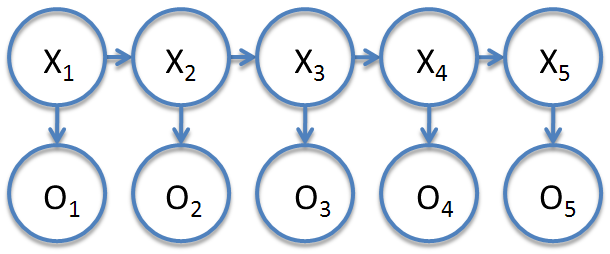
\includegraphics[scale=0.5]{images/hmm.png}\\
Elements to be determined in HMM are as follows:\\
\begin{itemize}
\item N, the number of hidden states in the model.
\item M, the number of distince observations symbols per state.
\item $A_{N\times N}$, the transition probability distribution, where $a_{ij} = \mathbf{Pr}(q_{t+1} =S_j|q_{t} = S_i)$, $1 \leq i, j \leq N$.
\item $B_{N\times M}$, the observation symbol probability distribution, where $b_j(k) = \mathbf{Pr}(O_t = v_k|q_t = S_j)$, $1\leq j\leq N, 1\leq k\leq M$
\item $\pi_{N\times 1}$, the initial state distribution, where $\pi_i = \mathbf{Pr}(q_1 = S_i)$, $1 \leq i \leq N$.
\end{itemize}
The $N$ and $M$ are pre-determined, could be selected by cross-validation. The rest consist the model parameter $\lambda = (A, B, \pi)$.\\\\
There are generally three basic problems in HMM: \\
\begin{itemize}
\item Problem 1: Compute the probability of the observation sequence $O$, given a model with parameter $\lambda $, $\mathbf{Pr}(O|\lambda)$.
\item Problem 2: Given the observation sequence $O$ and the model $\lambda$, choose a corresponding state sequence $Q$ which is optimal. 
\item Problem 3: Learn the model parameter $\lambda = (A,B,\pi)$, given the observation sequence $O$ to maximize $\mathbf{Pr}(O|\lambda)$.
\end{itemize}
In this project, in order to do gesture classification, we only need to solve problem 1 and problem 3.\\
\subsection {The forward-backward procedure}
To solve problem 1, we use a dynamic algorithm called forward-backward procedure briefly stated as following: \\
\emph{Forward procedure}\\
\begin{itemize}
\item Define $\alpha_t(i) = \mathbf{Pr}(O_1, O_2, ...,O_t, q_t = Si | \lambda)$.
\item Initialize $\alpha_1(i) = \pi_i b_i(O_1)$, $1 \leq i \leq N$.
\item Induction $\alpha_{t+1}(j) = \big[\sum_{j=1}^N \alpha_t(i)a_{ij}\big]b_j(O_{t+1})$, $1\leq t\leq T-1, 1\leq j\leq N$. (T is the length of the observation)
\end{itemize}
\emph{Backward procedure}\\
\begin{itemize}
\item Define $\beta_t(i) = \mathbf{Pr}(O_{t+1}, O_{t+2}, ...,O_T, q_t = Si | \lambda)$.
\item Initialize $\beta_T(i) = 1$, $1 \leq i \leq N$.
\item Induction $\beta_{t}(j) = \sum_{j=1}^N a_{ij}b_{j}(O_{t+1})\beta_{i+1}(j)$, $t = T-1, T-2, .., 1, 1\leq i\leq N$.
\end{itemize}
\emph{Outputs}
\begin{itemize}
\item $\mathbf{Pr}(O|\lambda) = \sum_{t,i} \alpha_t(i)\beta_i(O_t)$
\end{itemize}
The forward-backward dynamic programming algorithm achieves time complexity of $O(N^2T)$ in comparison with the brutal force approach's $O(TN^T)$.
\subsection {Baum-Welch method for training}
To solve problem 3, we used Baum-Welch method, which is equivalent to EM algorithm in HMM. \\\\
\emph{Declaration}
\begin{itemize}
\item Define $\xi_t(i,j) = \mathbf{Pr}(q_t = S_i, q_{t+1} = S_j| O, \lambda)$.
\item Define $\gamma_t(i) = \mathbf{Pr}(q_t = S_i| O, \lambda)$.
\end{itemize}
\emph{E-step}
\begin{itemize}
\item $\xi_t(i,j) = \frac{\alpha_t(i)a_{ij}b_j(O_{t+1})\beta_{t+1}(j)}{P(O|\lambda)}$.
\item $\gamma_t(i) = \sum_{j=1}^N \xi_t(i,j)$.
\end{itemize}
\emph{M-step}
\begin{itemize}
\item $\bar\pi = \gamma_1(i)$.
\item $\bar a_{ij} = \frac{\sum_{t=1}^{T-1} \xi_t(i,j)}{\sum_{t=1}^{T-1}\gamma_t(i)}$.
\item $\bar b_j(k) = \frac{\sum_{t=1, s.t. O_t = v_k}^T \gamma_t(j)}{\sum_t^T \gamma_t(j)}$.
\end{itemize}
Iterative execute the above algorithm until it converges to a local optima. 
\subsection {Scaling to prevent underflow}
HMM tends to underflow due to limited numerical precision of machine. We can handle this issue by scaling $\alpha$ and $\beta$. \\
\begin{align*}
\hat \alpha_t(i) = \frac{\alpha_t(i)}{\sum_{j=1}^N \alpha_t(j)}\\
\hat \beta_t(i) = \frac{\beta_t(i)}{\sum_{j=1}^N \beta_t(j)} \\
\end{align*}

\section {Training and Testing}
\subsection {Model selectoin and parameter initialization}
I used $N = 10$, $M =16$ for my submission, I determine $N$ and $M$ simply by trial and error. For the model parameter $\lambda = (A,B,\pi)$, I initialized them with random number and normalized each state. \\
\subsection {Training set and test set}
In the dataset, for each gesture, we are provided with 5 multiple gestures sequences, and 1 single gesture sequence. To train my models, \emph{I only used one sequence of each gesture}. And test it on the remaining 4 multiple sequences and 1 single sequence. \\
The following are the confusion matrix on the rest of multiple gestures, 93.33\%(28/30) of accuracy:\\
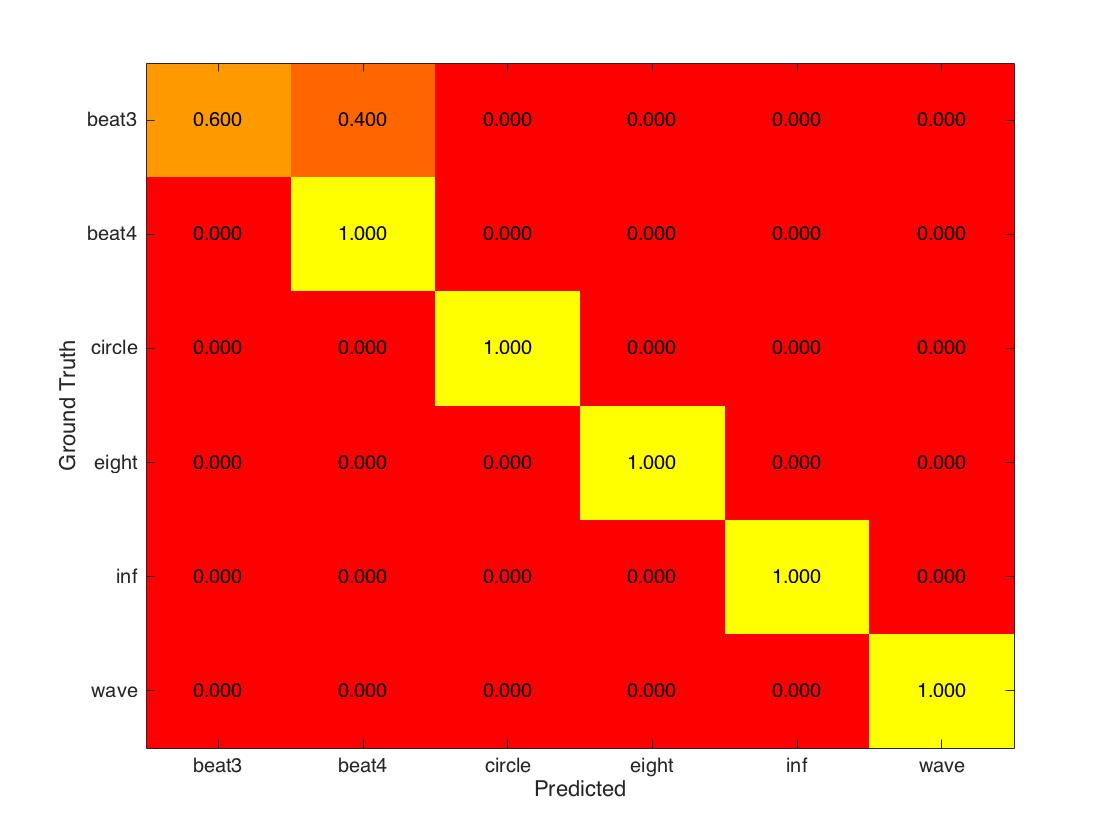
\includegraphics[width=\textwidth]{images/cfm.jpg}\\
Here are the results over the single gesture sequences, 91.67\%(11/12) accuracy:\\

\begin{center}
\begin{tabular}{|l|l|l|l|}
\hline
\# & Ground Truth & Prediction & Top Probability \\ \hline
1  & beat3        & beat4      & 0.4769          \\ \hline
2  & beat3        & beat3      & 0.5290          \\ \hline
3  & beat4        & beat4      & 0.6761          \\ \hline
4  & beat4        & beat4      & 0.6308          \\ \hline
5  & circle       & circle     & 0.8652          \\ \hline
6  & circle       & circle     & 0.8580          \\ \hline
7  & eight        & eight      & 0.9504          \\ \hline
8  & eight        & eight      & 0.9586          \\ \hline
9  & inf          & inf        & 0.6857          \\ \hline
10 & inf          & inf        & 0.6790          \\ \hline
11 & wave         & wave       & 0.4852            \\ \hline
12 & wave         & wave       & 0.4378            \\ \hline
\end{tabular}
\end{center}

\section {Calculate Probability}
In order to visualize the prediction results and obtain a clear estimation of prediction confidence, I use the follow procedure to transform the raw outputs of HMM prediction to probability. 
\begin{align*}
y_i =& \frac{log(\mathbf{Pr}(O|\lambda_i))}{\sum_i log(\mathbf{Pr}(O|\lambda_i))}\\
y_{min} =& min\{y_i\}\\
\hat y_i =& y_{min}/y_i \\
\mathbf{Pr}(Y = i|O) =& \hat y_i/\sum_i{\hat y_i} \\
\end{align*}
Where, $\mathbf{Pr}(O|\lambda_i)$ could be computed by forward-backward procedure, $\lambda_i$ is the model paramter for gesture $i$. $\mathbf{Pr}(Y = i|O)$ is the output probability that the gesture is $i$. \\
Below is an example visualization of the mis-classified single gesture \#1. We can see that the probabilities of gesture beat3 and beat4 are quite near to each other.\\
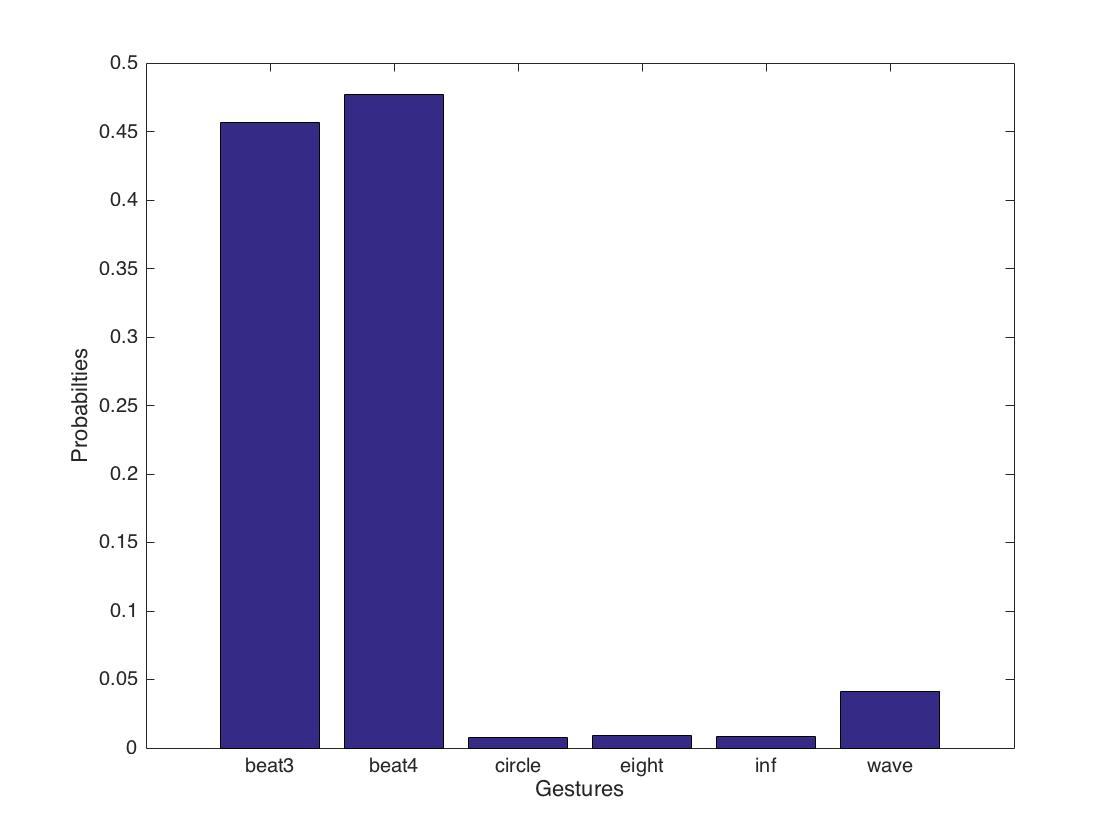
\includegraphics[width=\textwidth]{images/probs.jpg}\\
\section {Results and Discussion}
\subsection {Prediction on the validation test}
Here are the prediction results along with the probability distribution. On the validation set, my model achieved \emph{100\%} accuracy.\\
\begin{tabular}{|l|l|l|l|l|l|l|l|l|}
\hline
\# & beat3           & beat4           & circle          & eight           & inf             & wave            & Ground Truth & Prediction \\ \hline
1  & 0.4084          & 0.1469          & 0.0066          & 0.0120          & 0.0136          & \textbf{0.4125} & wave         & wave       \\ \hline
2  & 0.1630          & \textbf{0.7904} & 0.0070          & 0.0087          & 0.0073          & 0.0236          & beat4        & beat4      \\ \hline
3  & 0.0493          & 0.0260          & 0.0127          & 0.0867          & \textbf{0.7992} & 0.0261          & inf          & inf        \\ \hline
4  & \textbf{0.4971} & 0.4160          & 0.0093          & 0.0125          & 0.0112          & 0.0538          & beat3        & beat3      \\ \hline
5  & 0.0274          & 0.0269          & \textbf{0.8807} & 0.0288          & 0.0095          & 0.0268          & circle       & circle     \\ \hline
6  & 0.0285          & 0.0142          & 0.0075          & 0.0489          & \textbf{0.8866} & 0.0143          & inf          & inf        \\ \hline
7  & 0.0111          & 0.0081          & 0.0043          & \textbf{0.9580} & 0.0103          & 0.0082          & eight        & eight      \\ \hline
8  & 0.1915          & \textbf{0.7647} & 0.0065          & 0.0080          & 0.0067          & 0.0226          & beat4        & beat4      \\ \hline
\end{tabular}
\subsection {Discussion}
\begin{itemize}
\item Since in my project, the initialization of kmeans and parameter $\lambda$ are all random, also the 
Baum-Welch method could only achieve the local optima, there are some probability that we get bad model.
For the same configuration of parameters $N$ and $M$, I tried training multiple times to obtain a relatively optimal model.
\item I only used one sequence of each gesture for training with parameters $N=10$ and $M =16$, and it achieved 100\% prediction accuracy on validation set. I believe more training data will contribute to even more accurate prediction, in which case we might also need a more complex model to reduce the training bias. Due to limited computation power and time, I have not yet tried more complex models. 
\end{itemize}



\section {Acknowledgement}
Thanks Dr. Lee for designing and preparing this project and thanks TAs for timely responses to our questions.



\begin{thebibliography}{2} % Bibliography - this is intentionally simple in this template

\bibitem{Rabiner}
L.R.Rabiner, \emph{A tutorial on hidden markov models and selected apllications in speech recognition}. In A. Waibel and K.-F. Lee, editors, Readings in Speech Recognition, pages 267-296. Kaufmann, San Mateo, CA, 1990.

\bibitem{HMM520}
\emph{Hidden Markov Models}, CIS520 Machine Learning, University of Pennsylvania, https://alliance.seas.upenn.edu/~cis520/dynamic/2014/wiki/index.php?n=Lectures.HMMs


\end{thebibliography}


\end{document}